\documentclass{article}
\usepackage{graphicx} % Required for inserting images
\usepackage{listings}
\usepackage{xcolor}
\usepackage[hyphens]{url}
\usepackage{microtype}

\emergencystretch 3em
\let\oldtextunderscore\_
\renewcommand{\_}{\oldtextunderscore\allowbreak}

\lstset{
    language=Python,
    basicstyle=\ttfamily\footnotesize,
    keywordstyle=\color{blue}\bfseries,
    stringstyle=\color{red},
    commentstyle=\color{gray}\itshape,
    breaklines=true,
    showstringspaces=false,
    tabsize=4,
    frame=single
}


\title{Tamagotchi Wild Edition \\ Multi-Agent Care for Virtual Pets}
\author{Isabella Tagliafico}
\date{September 2026}

\begin{document}
\maketitle

\section*{Project Metadata and Proposal}

\begin{itemize}
    \item \textbf{Programming Languages Used:} Python 3.12, AgentSpeak(L)
    \item \textbf{Libraries Used:} SPADE (v4.1.4), SPADE-BDI (v0.3.2), NiceGUI (v3.15.0), pytest (v9.1.1)
    \item \textbf{Project Difficulty:} Hard
\end{itemize}

\subsection*{Initial Project Proposal}
The project proposes an automated management system for a Wildlife Rescue Center (CRAS), a domain derived from my direct experience as an ENPA volunteer.
The implementation foresees a 2D grid visualization, adopting the architecture from the cleaning-robots (MarsEnv) example in Jason. 
Alternatively, the adoption of the JaCaMo framework will be evaluated should the initial approach require a higher level of abstraction.

Environment ModelingThe environment is modeled as a grid partitioned into specific functional areas: Food Storage, Medical Storage, Cage Area, and Treatment Room. Within this space, wild animals are represented as passive objects (resources) upon which the agents operate.

Agent Architecture and DevelopmentThe system will orchestrate three types of agents (N Veterinarians, N Feeding Staff, N Logistics Staff).
Development will follow an incremental approach: starting with the implementation of the feeding logic to validate basic cooperation mechanisms, and subsequently integrating care and health management routines.

Role Specifications:Veterinary Agent: Manages healthcare logic. 
It interacts with the Treatment Room and Medical Storage; it coordinates the workflow by sending requests to the Logistics Agent for patient transfer to the care area.Feeding Agent: Provides for animal sustenance. It interacts with the Food Storage; its activation is triggered by a request from the Logistics Agent (e.g., filling bowls).Logistics Agent (Transport): Manages the physical movement of the animal between the Treatment Room and the Cage Area. It is triggered by the Veterinary Agent when an animal requires transport, and it triggers the Feeding Agent to replenish food bowls in the cages.

As an advanced objective, the project envisages the implementation of concurrency control policies governing access to shared resources (operational areas). This mechanism will enforce capacity constraints (e.g., a maximum of 2 concurrent agents), contingent upon the consolidation of the system's core functionalities.

\bigskip
\hrule
\bigskip

\section{Introduction}
This project stems from the work developed for the Natural Language Processing 
course, reinterpreting the same domain (a Wildlife Rescue Center CRAS)
using a multi-agent architecture. The facility is divided into four operational areas: 
Cage Area, Food Storage, Medical Storage, and Treatment Room. Inside it, 
veterinarians, logistics staff, and feeding personnel must coordinate in real 
time while respecting precise physical constraints. Each area admits at most 
two operators simultaneously; the treatment room adds a further constraint, 
allowing up to three animals on the examination table at once, with each 
logistics operator limited to transporting a single patient at a time.
The system is developed in Python 3.12 with a distributed multi-agent 
architecture based on SPADE (Smart Python Agent Development Environment, 
v4.1.4), which manages the agent lifecycle and asynchronous communication over 
the XMPP network. The deliberative component of the operators is implemented 
through the SPADE-BDI extension (v0.3.2), which realizes the 
Belief-Desire-Intention cognitive model via the AgentSpeak interpreter. 
Real-time monitoring is handled by NiceGUI (v3.15.0), which generates a 
web dashboard accessible from the browser.


\section{Incremental Development Methodology and System Implementation}
The development approach of the project was incremental, as there were multiple architectural layers to address.
\subsection{Phase 0: Compatibility Study}
Initially, lacking certainty that the chosen libraries (Python 3.12, SPADE for the XMPP network, and the BDI interpreter for AgentSpeak) were fully compatible with each other, it was decided to build a disposable minimal prototype with two agents to verify their integration. A command-line smoke test was then executed to confirm that the local XMPP server started and responded correctly.
\subsection{Phase 1: Foundation of Domain and Environment}
Before introducing any agent, the physical model of the world was implemented, defining what actions are possible and under what conditions. The following components were built:
\begin{itemize}
    \item the $12 \times 8$ grid with the geometric subdivision into four areas (Food Storage, Medical Storage, Cage Area, Treatment Room);
    \item the base entities (\texttt{Position}, \texttt{Animal}, \texttt{Cage}, \texttt{Bowl}, food stocks, medicine stocks) and the \texttt{EnvironmentState} controller.
\end{itemize}
This phase was fundamental because it allowed building the physical and mathematical foundations of the world in pure Python, without yet introducing SPADE, the XMPP network, or BDI logic.
In this phase, the following modules were written:
\begin{itemize}
    \item \textbf{\texttt{domain/entities.py}}, where the base data structures were defined:
    \begin{itemize}
        \item \texttt{Position(x, y)}: integer coordinates on the grid;
        \item \texttt{Area}: rooms with their cell perimeters and respective capacities;
        \item \texttt{Animal}, \texttt{Cage}, \texttt{Bowl}: physical objects with unique identifiers;
        \item \texttt{HealthStatus}: finite health states (\texttt{HEALTHY}, \texttt{HUNGRY}, \texttt{SICK}, \texttt{IN\_TREATMENT}, \texttt{TREATED}, \texttt{IN\_OUTBOUND\_TRANSPORT}, \texttt{IN\_RETURN\_TRANSPORT}, \texttt{READY\_FOR\_TRANSPORT}).
    \end{itemize}
    \item \textbf{\texttt{environment/state.py}}: The \texttt{EnvironmentState} class was created to model the physical space and the laws of the world. It maintains the ground truth of all entities: the positions of animals, coordinates of obstacles, bowl levels, and quantities of food and medicine stocks. Furthermore, it validates physical actions, verifying whether an action attempted by an operator is permitted according to the world rules. It is a passive component: it makes no autonomous decisions and possesses no goals, beliefs, or desires; in summary, it represents the simulated physical environment (the ground truth).
\end{itemize}
Unit tests were written to validate each world rule before moving on.
\subsection{Phase 2: Agent Creation and Initial Workflow (Feeding)}
In this phase, the first real SPADE agents were created, connected to the XMPP network and guided by BDI logical plans. Following the incremental methodology, it was decided not to implement the complete system immediately, but to validate execution starting from a single hungry animal with a single empty bowl. Notably, agents represent the staff operators of the center, whereas animals are not agents but passive physical objects.
In this phase, the following entities were created:
\begin{itemize}
    \item 1 \texttt{EnvironmentAgent} (the centralized environment arbiter);
    \item 1 \texttt{LogisticsAgent} (the coordinator);
    \item 1 \texttt{FeedingAgent} (the operational executor);
    \item 1 cage with 1 empty bowl and the storage room with food stocks.
\end{itemize}
To initially verify baseline operations, the following aspects were temporarily excluded:
\begin{itemize}
    \item the presence of veterinarians and medical treatments;
    \item the presence of duplicate operators (only a single agent per role);
    \item room capacity constraints (no waiting queues at room entrances);
    \item the graphical interface (operating solely via terminal logs).
\end{itemize}
What was implemented:
\begin{enumerate}
    \item \textbf{The initial BDI plans (\texttt{.asl})}:
    \begin{itemize}
        \item \texttt{logistics.asl}: receives the \texttt{bowl\_empty} belief and adopts the plan to assign it to the feeding operator;
        \item \texttt{feeding.asl}: receives the \texttt{feeding\_task} belief and triggers the \texttt{complete\_feeding} operational plan.
    \end{itemize}
    \item \textbf{The FIPA message chain via XMPP}:
    \begin{itemize}
        \item The \texttt{EnvironmentAgent} sends a perception message to the \texttt{LogisticsAgent} informing it that the bowl in the cage is empty;
        \item The \texttt{LogisticsAgent} sends a request to the \texttt{FeedingAgent} specifying the task to be performed;
        \item The \texttt{FeedingAgent} accepts the task: it requests permission from the environment to withdraw food from the stocks (which are decremented from the total) and subsequently requests the action to refill the bowl, whose level is updated to 1 by the environment to record full availability;
        \item The \texttt{FeedingAgent} finally notifies the \texttt{LogisticsAgent} of the successful completion of the task.
    \end{itemize}
\end{enumerate}
Dedicated tests were also created in this phase to verify that all operations functioned correctly.
\subsection{Phase 3: Medical Treatment and Transport}
Phase 3 introduced higher complexity, involving the initial forms of cooperation between heterogeneous agents. An animal cannot move autonomously from the cage area to the treatment room; therefore, the intervention of an operator was required for transportation. Furthermore, for the administration of medical treatments, it was essential to introduce the Veterinary agent role.
What was implemented in Phase 3:
\begin{itemize}
    \item \textbf{The \texttt{VeterinaryAgent} and its BDI plan (\texttt{veterinary.asl})}: introduces the specialized medical agent, which receives notifications of sick animals, requests transport from logistics, retrieves medicine from medical storage, and administers treatment in the treatment room.
    \item \textbf{The transport role of the \texttt{LogisticsAgent}}: the logistics operator takes on the task of transporting the animal from the Cage Area to the Treatment Room and vice versa. It is triggered directly by the veterinary agent for both outbound and return transport.
    \item \textbf{The animal finite state machine}: the animal does not heal instantaneously, but traverses a strict sequence of 6 physical states verified by the \texttt{EnvironmentAgent}:
    \begin{itemize}
        \item \texttt{SICK}: sick inside its cage (it cannot be treated there);
        \item \texttt{IN\_OUTBOUND\_TRANSPORT}: picked up by the logistics operator and traveling toward the treatment room (no other agent can interact with it);
        \item \texttt{IN\_TREATMENT}: placed on the examination table in the treatment room awaiting the doctor;
        \item \texttt{TREATED}: treated with the drug by the veterinarian, but still on the table;
        \item \texttt{IN\_RETURN\_TRANSPORT}: picked up again by the logistics operator for the return trip;
        \item \texttt{HEALTHY}: returned to its cage of origin, healed and free.
    \end{itemize}
    \item \textbf{Physical clinical constraints}:
    \begin{itemize}
        \item table capacity: a maximum of 3 patients simultaneously in the treatment room;
        \item carrying capacity: each logistics operator can carry only one animal at a time;
        \item medication precondition: the veterinarian cannot perform the treatment without first retrieving the dose from the Medical Storage.
    \end{itemize}
\end{itemize}
Specific tests were also executed for this phase to ensure correct behavioral execution.
\subsection{Phases 4 and 5: Scalability and Concurrency}
This part addressed the final and most complex challenge: scaling the number of animals and operators while managing concurrency. In earlier phases (Phases 2 and 3), management was simplified by having a single agent per role.
With multiple agents, fundamental logistical issues emerged:
\begin{itemize}
    \item \textbf{Task contention (\textit{Race Condition})}: two operators attempting to perform the same task simultaneously (e.g., refilling the same bowl).
    \item \textbf{Physical bottleneck (\textit{Overcrowding and Deadlock})}: operators attempting to enter the same room at the same time, blocking each other.
\end{itemize}
In \textbf{Phase 4}, runtime configuration was implemented to select the number of animals (up to a maximum of 40) and operators (up to a maximum of 15). Dynamic world generation was also introduced: launching 5 animals, for instance, automatically instantiates 5 cages, 5 distinct animal species, and 10 independent tasks. Finally, the Round-Robin algorithm was adopted to distribute tasks evenly among all available operators (e.g., with 3 feeding operators and 6 bowls, each operator takes charge of 2).
\textbf{Phase 5} introduced concurrency management and mutual exclusion:
\begin{itemize}
    \item \textbf{Atomic task reservation (\texttt{CLAIM\_TASK})}: prior to initiating any action, the operator must register the task with the \texttt{EnvironmentAgent}. The first agent to arrive acquires the lock; if a second agent requests the same task, the environment rejects it, signaling that the work has already been assigned to another operator.
    \item \textbf{Room semaphores (\texttt{ACQUIRE\_AREA} and \texttt{RELEASE\_AREA})}: each room (Food Storage, Medical Storage, Treatment Room, Cage Area) admits a maximum of 2 occupants simultaneously.
    \item \textbf{Asynchronous retry loop (\textit{Deadlock Prevention})}: if an operator requests access to an area where 2 colleagues are already present, the environment replies with \texttt{accepted=False}. The operator does not block or terminate execution: it enters a short asynchronous pause (\texttt{await asyncio.sleep(0.05)}) and retries requesting entry until one of the two occupants exits and issues \texttt{RELEASE\_AREA}.
\end{itemize}
Dedicated tests were also established in this phase to verify that the concurrent workflow operated without anomalies.
\subsection{Phase 6: Graphical User Interface Implementation}
In a distributed multi-agent system communicating via XMPP, tracking the progression of actions solely through terminal log lines proved impractical. A graphical user interface was therefore developed to make the simulation observable in real time; the frontend code was built with the aid of generative AI tools.
The \texttt{VisualizationAgent} was therefore created, acting as a passive camera that receives state snapshots from the environment. The bridge module \texttt{gui\_bridge.py} was then implemented to transmit data to the NiceGUI web server, which renders the interactive SVG map in real time, displaying operator movements and status updates dynamically.

\section{Domain Modeling and Physical Environment}
This section formalizes the spatial layout and the physical rules governing the rescue center. The domain model is implemented in pure Python, completely decoupled from network messaging (SPADE/XMPP), BDI reasoning, and graphical rendering.
\subsection{Domain Entities (\texttt{domain/entities.py})}
All physical elements of the center are modeled using immutable classes (\texttt{@dataclass(frozen=True)}), in order to prevent accidental modifications and ensure safety among concurrent tasks:
\begin{itemize}
    \item \textbf{Space and Rooms}: The world is a grid of coordinates \texttt{Position(x, y)} of size $12 \times 8$, divided into four closed areas (\texttt{Area}): \textit{Food Storage}, \textit{Medical Storage}, \textit{Cage Area}, and \textit{Treatment Room}.
    \item \textbf{Objects and Resources}: Cages (\texttt{Cage}) and bowls (\texttt{Bowl}) are located at fixed points on the map. Stocks of food (\texttt{FoodStock}) and medicines (\texttt{MedicineStock}) keep track of the numerical quantities remaining in the storages.
    \item \textbf{Animal Life Cycle (\texttt{HealthStatus})}: The domain enumeration defines eight states (including \texttt{HUNGRY} for feeding and \texttt{READY\_FOR\_TRANSPORT} for pre-transit staging), but the medical recovery cycle enforced by the environment follows a mandatory sequence of six physical states:
\begin{center}
\small
\texttt{SICK} $\rightarrow$ \texttt{IN\_OUTBOUND\_TRANSPORT} $\rightarrow$ \texttt{IN\_TREATMENT} \\
$\rightarrow$ \texttt{TREATED} $\rightarrow$ \texttt{IN\_RETURN\_TRANSPORT} $\rightarrow$ \texttt{HEALTHY}
\end{center}
\end{itemize}
\subsection{Actions and Contracts (\texttt{domain/actions.py})}
Agents cannot directly touch the world data: to do anything they must send a formal request:
\begin{itemize}
    \item \textbf{Action Types (\texttt{ActionType})}: An enumeration of 15 permitted domain operations, including reserving tasks (\texttt{CLAIM\_TASK}), entering or leaving rooms (\texttt{ACQUIRE\_AREA}, \texttt{RELEASE\_AREA}), managing resources (\texttt{TAKE\_FOOD}, \texttt{TAKE\_MEDICINE}, \texttt{FILL\_BOWL}), and executing medical stages (\texttt{PICKUP\_SICK\_ANIMAL}, \texttt{DELIVER\_TO\_TREATMENT}, \texttt{TREAT\_ANIMAL}, \texttt{PICKUP\_TREATED\_ANIMAL}, \texttt{RETURN\_ANIMAL\_TO\_CAGE}).
    \item \textbf{Commands and Outcomes (\texttt{ActionCommand} and \texttt{ActionResult})}: For each requested action, the environment responds atomically stating whether it was accepted (\texttt{accepted = True}) or rejected (\texttt{accepted = False}), always specifying the reason for rejection.
\end{itemize}
\subsection{Authoritative Environment (\texttt{environment/state.py})}
The \texttt{EnvironmentState} class is the only true custodian of the state of the world (\textit{ground truth}). It does not reason and makes no decisions: it only checks that physical rules are respected before executing any modification:
\begin{itemize}
    \item \textbf{Room Capacity Rule}: In each room there can be at most two operators at the same time. If a room is already full, the environment rejects entry and the agent waits outside until a spot is freed.
    \item \textbf{Clinical and Transport Rules}: On the examination table of the treatment room there can be at most three animals simultaneously, and each logistics operator can transport only one animal at a time.
    \item \textbf{History and Snapshots}: At each valid action, the environment assigns a progressive number to the event and creates an exact, protected copy of the state (\texttt{WorldSnapshot}), which is then sent to the graphical screen without risking altering the simulation data.
\end{itemize}

\section{Multi-Agent System Architecture}
Within the project, a total of five distinct types of agents operate. They are not all built the same way: three of them (\texttt{VeterinaryAgent}, \texttt{LogisticsAgent}, \texttt{FeedingAgent}) are cognitive BDI agents : they maintain an internal belief base, adopt goals, and deliberate through AgentSpeak plans before acting. The remaining two (\texttt{EnvironmentAgent} and \texttt{VisualizationAgent}) are purely reactive: they hold no beliefs and make no decisions, but simply respond to incoming messages according to fixed rules.
\begin{itemize}
    \item \texttt{EnvironmentAgent} — reactive, no BDI
    \item \texttt{LogisticsAgent} — BDI cognitive operator
    \item \texttt{FeedingAgent} — BDI cognitive operator
    \item \texttt{VeterinaryAgent} — BDI cognitive operator
    \item \texttt{VisualizationAgent} — reactive, no BDI
\end{itemize}

\subsection{EnvironmentAgent}
\begin{itemize}
    \item \textbf{Role}: Acts as the XMPP communication bridge between the physical world model (\texttt{EnvironmentState}) and the multi-agent network.
    \item \textbf{Architecture}: It is a reactive SPADE agent implemented in pure Python. Unlike the other agents, it does not employ the BDI paradigm: its behavior is purely deterministic and reactive, limited to receiving requests and verifying their compliance against the physical rules of the world.
\end{itemize}
\subsubsection{Operational Example}
\begin{itemize}
    \item If an operator asks: \textit{"Can I take a dose of medicine?"}, the Environment does not engage in complex deliberation: it deterministically checks whether the remaining stock is greater than zero. If so, it responds positively and decrements the stock by one dose; otherwise, it rejects the request.
    \item If an operator asks: \textit{"Can I enter the treatment room?"}, the Environment checks whether the current number of occupants is below maximum capacity: if so, it approves access; otherwise, it rejects it.
\end{itemize}
\subsubsection{Core Responsibilities}
\begin{itemize}
    \item Receives physical action requests sent by operators (\texttt{ActionRequest}) and responds by accepting or rejecting them in compliance with the laws of the world;
    \item Acts as a sensor for the facility: monitors the state of the center and sends perception notifications to designated agents according to the FIPA standard (e.g., notifying Logistics of an empty bowl or the Veterinarian of a sick animal);
    \item Transmits state update snapshots to the \texttt{VisualizationAgent};
    \item Ensures simulation integrity, preventing the execution of any unlawful or physically impossible action.
\end{itemize}
\subsubsection{Physical Request Processing}
The management logic for physical actions is defined within the module \texttt{src/tamagotchi\_wild/agents/environment\_agent.py}:
\begin{lstlisting}[language=Python, caption={Physical action request processing in \texttt{environment\_agent.py}}]
def process_action_request(world: EnvironmentState, body: str) -> ActionResponse:
    try:
        request = ActionRequest.from_json(body)
    except MessageContractError as exc:
        return ActionResponse(
            task_id="unknown",
            accepted=False,
            reason=str(exc),
            event_sequence=None,
        )
    return ActionResponse.from_result(
        request.task_id, world.apply(request.to_command())
    )
\end{lstlisting}
This function illustrates the primary workflow: the agent receives the message body, deserializes it into a structured request object, and forwards it to the physical environment (\texttt{world.apply}), returning a response that specifies whether the action was accepted or rejected with the corresponding reason.
\subsubsection{Reception Cycle and FIPA-ACL Interaction}
The asynchronous cycle that receives and manages requests is implemented via SPADE's cyclic behavior (\texttt{RequestBehaviour}):
\begin{lstlisting}[language=Python, caption={Asynchronous FIPA-ACL request handling in \texttt{RequestBehaviour}}]
class RequestBehaviour(CyclicBehaviour):
    async def run(self) -> None:
        message = await self.receive(timeout=1)
        if message is None:
            return
        request = None
        try:
            request = ActionRequest.from_json(message.body)
        except MessageContractError:
            pass
        response_data = process_action_request(self.agent.world, message.body)
        response = Message(to=str(message.sender))
        conversation_id = message.get_metadata("conversation-id")
        response.thread = message.thread or conversation_id
        response.set_metadata(
            "performative", "inform" if response_data.accepted else "failure"
        )
        response.set_metadata("ontology", ENVIRONMENT_ONTOLOGY)
        response.set_metadata("language", MESSAGE_LANGUAGE)
        if conversation_id:
            response.set_metadata("conversation-id", conversation_id)
        response.body = response_data.to_json()
        await self.send(response)
\end{lstlisting}
This behavior constitutes the asynchronous cycle that processes operator requests and formalizes communication using the \textbf{FIPA-ACL} standard (Foundation for Intelligent Physical Agents - Agent Communication Language), which regulates the format and intentionality of inter-agent messages.
The FIPA standard specifies various communicative performatives (including \texttt{request}, \texttt{inform}, \texttt{failure}, and \texttt{agree}). In the responses of the \texttt{EnvironmentAgent}, only \texttt{inform} and \texttt{failure} labels are used:
\begin{itemize}
    \item \textbf{\texttt{inform}}: notifies the agent of the successful application of the action in the real world.
    \item \textbf{\texttt{failure}}: notifies the agent of the rejection of the attempted action (for instance, when requested resources are exhausted or room access is saturated).
\end{itemize}
The \texttt{EnvironmentAgent} does not use the \textbf{\texttt{agree}} performative. An \texttt{agree} message denotes formal acceptance of a task requiring deferred execution over time, as observed in operational agents like the \texttt{FeedingAgent}. In contrast, the environment validates and executes actions atomically and instantaneously, making an intermediate execution promise redundant.
\subsubsection{Sensory Perception Triggers}
In addition to passive request handling, the \texttt{EnvironmentAgent} acts proactively as a sensor for the facility through two methods dedicated to signaling hunger and animal illness:
\begin{lstlisting}[language=Python, caption={Perception publishing methods in \texttt{EnvironmentAgent}}]
async def publish_bowl_empty(
    self,
    recipient: str,
    task_id: str,
    cage_id: str,
    bowl_id: str,
    timeout_seconds: float = 5.0,
) -> None:
    sent = asyncio.Event()
    self.add_behaviour(
        self.PerceptionSender(
            recipient,
            BowlEmptyPerception(task_id, cage_id, bowl_id),
            sent,
        )
    )
    await asyncio.wait_for(sent.wait(), timeout=timeout_seconds)
async def publish_sick_animal(
    self,
    recipient: str,
    task_id: str,
    animal_id: str,
    cage_id: str,
    timeout_seconds: float = 5.0,
) -> None:
    sent = asyncio.Event()
    self.add_behaviour(
        self.SickAnimalSender(
            recipient,
            SickAnimalPerception(task_id, animal_id, cage_id),
            sent,
        )
    )
    await asyncio.wait_for(sent.wait(), timeout=timeout_seconds)
\end{lstlisting}
These two methods serve as sensory alarms, signaling respectively an empty bowl condition and the detection of a sick animal. From a technical perspective, both methods share the same operational mechanism:
\begin{enumerate}
    \item Instantiate and attach a temporary, disposable SPADE behavior (\texttt{OneShotBehaviour}, namely \texttt{PerceptionSender} and \texttt{SickAnimalSender});
    \item Serialize the details of the perceptual event into JSON format within an XMPP message carrying the FIPA performative \texttt{inform};
    \item Transmit the message to the designated recipient across the XMPP network;
    \item Via the instruction \texttt{await asyncio.wait\_for(sent.wait())}, suspend execution pending confirmation of successful message transmission before proceeding.
\end{enumerate}



\subsection{FeedingAgent}
\subsubsection{Role and Nature of the Agent}
The \texttt{FeedingAgent} is the operational staff member responsible for the sustenance of hospitalized animals. Its fundamental purpose is to refill empty bowls while ensuring resource consistency and preventing operational conflicts with other colleagues.
Unlike the \texttt{EnvironmentAgent} (which is a reactive controller without deliberative capabilities), the \texttt{FeedingAgent} adopts a two-tier hybrid architecture:
\begin{itemize}
    \item The high-level deliberative tier models reasoning and mental states via the BDI architecture written in AgentSpeak(L);
    \item The low-level executive tier manages distributed communication, asynchronous actions, and physical interaction in the world via Python and the SPADE platform.
\end{itemize}
\subsubsection{Interlocutors}
The agent constantly communicates with only two entities in the system:
\begin{itemize}
    \item \textbf{With the \texttt{LogisticsAgent}}:
    \begin{itemize}
        \item Receives task assignments via FIPA messages with the \texttt{request} performative (\textit{"Refill the bowl in cage X"});
        \item Responds by sending a FIPA \texttt{agree} message (to confirm the start of work), \texttt{refuse} (if the task has already been taken by another operator), or \texttt{inform} (to notify that the bowl has been successfully refilled).
    \end{itemize}
    \item \textbf{With the \texttt{EnvironmentAgent}}:
    \begin{itemize}
        \item Communicates via the \texttt{cras.environment} ontology to validate physical actions: requests exclusive task reservation, room access and release, food retrieval from storage, and pouring into the bowl.
    \end{itemize}
\end{itemize}
\subsubsection{Complete Operational Cycle}
The life cycle of each feeding task is carried out in six linear steps:
\begin{enumerate}
    \item \textbf{Reception}: the agent intercepts the service order from Logistics containing the cage ID and bowl ID.
    \item \textbf{Atomic Task Reservation}: before moving, it contacts the Environment to acquire the lock on the task. If a colleague has already taken charge of the same bowl, it responds to the \texttt{LogisticsAgent} with \texttt{refuse}. If it acquires the lock, it starts the plan.
    \item \textbf{Acceptance}: sends a formal \texttt{agree} message to the \texttt{LogisticsAgent} to formally commit to executing the task.
    \item \textbf{Stock Retrieval and Verification}: moves to the Food Storage, enters respecting the capacity limit, and attempts the \texttt{TAKE\_FOOD} action. The Environment verifies stock: if the quantity is sufficient, it decrements the storage; otherwise, the action fails due to resource exhaustion and the task is aborted.
    \item \textbf{Bowl Refilling}: reaches the assigned cage in the Cage Area and executes the \texttt{FILL\_BOWL} action.
    \item \textbf{Closure}: sends the final FIPA \texttt{inform} message to Logistics to declare task completion and updates its internal belief base.
\end{enumerate}
\subsubsection{Tier Separation: Beliefs File (.asl) vs. Python File (.py)}
To avoid confusion between the theoretical plan and practical execution, the agent is clearly separated into two files:
\paragraph{The Beliefs File: \texttt{src/tamagotchi\_wild/bdi/feeding.asl}}
This component encapsulates the declarative deliberative layer of the agent. It performs no numerical computation or network I/O; its role is confined to managing the belief base, adopting goals, and executing plans.
\begin{lstlisting}
!boot.
+!boot <-
    .mark_bdi_ready.
+feeding_task(TaskId, CageId, BowlId) <-
    !complete_feeding(TaskId, CageId, BowlId).
+!complete_feeding(TaskId, CageId, BowlId) <-
    .execute_feeding(TaskId, CageId, BowlId).
+feeding_succeeded(TaskId) <-
    .record_feeding_outcome(TaskId, completed).
+feeding_failed(TaskId) <-
    .record_feeding_outcome(TaskId, failed).
\end{lstlisting}
\begin{itemize}
    \item \textbf{Initialization}: the \texttt{!boot} goal starts the agent and notifies the system that the logical engine is ready (\texttt{.mark\_bdi\_ready});
    \item \textbf{Reaction to event}: acquiring the \texttt{+feeding\_task} belief triggers the \texttt{!complete\_feeding} plan, which delegates the physical action to the Python module by calling \texttt{.execute\_feeding};
    \item \textbf{Conclusion}: the returning beliefs \texttt{+feeding\_succeeded} or \texttt{+feeding\_failed} formally record the final outcome in the agent's mind.
\end{itemize}
\paragraph{The Python Executive File: \texttt{feeding\_agent.py}}
The \texttt{feeding\_agent.py} module constitutes solely the executive component of the agent: it makes no autonomous decisions, but translates what the BDI plan has established into physical actions and network messages.
The material execution is encapsulated in the \texttt{\_execute} method of the \texttt{ExecuteFeeding} class:
\begin{lstlisting}
class ExecuteFeeding(CyclicBehaviour):
    async def _execute(self) -> None:
        requester = self.agent.task_requesters[self.task_id]
        await self._send_status(requester, "agree", "accepted")
        self.agent.activity_log.record(
            self.task_id,
            self.agent.agent_label,
            "task_accepted",
        )
        take_result = await self._perform_in_area(
            self.agent.food_area_id,
            self.agent.food_position,
            ActionType.TAKE_FOOD,
            self.agent.food_stock_id,
            1,
        )
        if not take_result.accepted:
            await environment_action(
                self,
                self.task_id,
                ActionType.FAIL_TASK,
                self.task_id,
            )
            await self._fail(requester, take_result.reason)
            return
        fill_result = await self._perform_in_area(
            self.agent.cage_area_id,
            self.agent.bowl_position,
            ActionType.FILL_BOWL,
            self.bowl_id,
            1,
        )
        if not fill_result.accepted:
            await self._fail(requester, fill_result.reason)
            return
        await self._send_status(requester, "inform", "completed")
        self.agent.activity_log.record(
            self.task_id,
            self.agent.agent_label,
            "task_completed",
        )
        self.agent.bdi.set_belief("feeding_succeeded", self.task_id)
\end{lstlisting}
Unlike the \texttt{EnvironmentAgent} (which applied instantaneous actions and responded solely with \texttt{inform} or \texttt{failure}), this code clearly illustrates the sequential adoption of two distinct FIPA performatives, necessary for a task that develops over time:
\begin{itemize}
    \item \textbf{\texttt{agree}}: sent immediately to the \texttt{LogisticsAgent} to confirm formal commitment to the task;
    \item \textbf{\texttt{inform}}: sent at the end to certify that the bowl is full, closing the cycle with the update of the internal belief.
\end{itemize}


\subsection{LogisticsAgent}
\subsubsection{Role and Nature of the Agent}
The \texttt{LogisticsAgent} is the operational coordinator of the facility and the physical carrier responsible for animal transportation. Its purpose is twofold: to balance and dispatch feeding tasks among available operators and to manage the transport of patients between the cage area and the treatment room.
Like the \texttt{FeedingAgent}, it adopts a two-tier hybrid architecture combining BDI logic in AgentSpeak for decision-making and SPADE in Python for networking:
\begin{itemize}
    \item While the \texttt{FeedingAgent} is a pure operational executor, the \texttt{LogisticsAgent} combines both coordination (assigning food tasks to others) and direct physical action (personally transporting animals).
\end{itemize}
\subsubsection{Interlocutors}
The agent communicates with three entities:
\begin{itemize}
    \item \textbf{With the \texttt{EnvironmentAgent}}:
    \begin{itemize}
        \item Receives sensor notifications regarding empty bowls;
        \item Validates physical actions: requests task reservation, animal pickup from the cage, delivery to the treatment room, and return maneuvers.
    \end{itemize}
    \item \textbf{With the \texttt{FeedingAgent}}:
    \begin{itemize}
        \item Dispatches replenishment orders via FIPA messages with the \texttt{request} performative;
        \item Receives \texttt{agree}, \texttt{refuse}, or \texttt{inform} replies from the feeding operator.
    \end{itemize}
    \item \textbf{With the \texttt{VeterinaryAgent}}:
    \begin{itemize}
        \item Receives transport requests for outbound transit to the treatment room or return to the cage;
        \item Responds confirming commitment via \texttt{agree}, signaling possible failures with \texttt{failure}, or notifying completed delivery with \texttt{inform}.
    \end{itemize}
\end{itemize}
\subsubsection{Complete Operational Cycle}
The agent manages two operational workflows:
\paragraph{Workflow A: Feeding Coordination}
\begin{enumerate}
    \item \textbf{Reception}: receives the empty bowl alert from the Environment;
    \item \textbf{Dispatching}: uses the Round-Robin algorithm to select an available feeding operator and evenly distribute the workload;
    \item \textbf{Assignment}: sends the request to the operator, waits for acceptance, and receives the final completion notification.
\end{enumerate}
\paragraph{Workflow B: Medical Transport of Animals}
\begin{enumerate}
    \item \textbf{Order Reception}: the Veterinarian requests transport of a patient for outbound or return transit;
    \item \textbf{Atomic Task Reservation}: contacts the Environment to lock the task and prevent colleagues from overlapping;
    \item \textbf{Acceptance}: sends an \texttt{agree} message to the Veterinarian to confirm the start of transit;
    \item \textbf{Animal Pickup}: reaches the starting location and takes custody of the animal (only one at a time);
    \item \textbf{Delivery}: transports the animal to its destination (on the examination table or in the origin cage after treatment);
    \item \textbf{Closure}: sends the final \texttt{inform} message to the Veterinarian to certify completed delivery.
\end{enumerate}
\subsubsection{Tier Separation: Beliefs File (.asl) vs. Python File (.py)}
The agent is clearly separated between logical mind and material execution:
\paragraph{The Beliefs File: \texttt{src/tamagotchi\_wild/bdi/logistics.asl}}
Unlike the \texttt{FeedingAgent} (which holds a single belief for a task it executes entirely on its own), the BDI mind of the \texttt{LogisticsAgent} manages two profoundly different types of beliefs:
\begin{itemize}
    \item \textbf{Feeding coordination beliefs}: upon receiving the empty bowl notification, it does not act directly but triggers a plan to delegate the work to a feeding operator;
    \item \textbf{Medical transport beliefs}: handles requests from the Veterinarian, logically distinguishing between outbound transit toward the treatment room and return transit to the cage of origin.
\end{itemize}
\begin{lstlisting}
!boot.
+!boot <-
    .mark_bdi_ready.
+bowl_empty(TaskId, CageId, BowlId) <-
    !ensure_food(TaskId, CageId, BowlId).
+!ensure_food(TaskId, CageId, BowlId) <-
    .request_feeding(TaskId, CageId, BowlId).
+feeding_completed(TaskId) <-
    .finish_feeding_workflow(TaskId, completed).
+feeding_failed(TaskId) <-
    .finish_feeding_workflow(TaskId, failed).
+transport_requested(TaskId, AnimalId, CageId, outbound) <-
    .execute_transport(TaskId, AnimalId, CageId, outbound).
+transport_requested(TaskId, AnimalId, CageId, return) <-
    .execute_transport(TaskId, AnimalId, CageId, return).
\end{lstlisting}
\begin{itemize}
    \item \textbf{Initialization}: certifies that the decision engine is ready;
    \item \textbf{Food dispatching}: transforms the hunger belief into an order to send to an operator;
    \item \textbf{Transport execution}: transforms the Veterinarian's request into the physical action of animal movement;
    \item \textbf{Conclusion}: records the final outcome in agent memory.
\end{itemize}
\paragraph{The Python Executive File: \texttt{logistics\_agent.py}}
The Python class \textbf{\texttt{LogisticsAgent}} manages the dual operational role of the agent: dispatching feeding tasks and physically moving animals in the field.
The internal architecture is organized into five components:
\begin{itemize}
    \item \textbf{Alarms and Food Claim} (\textbf{\texttt{PerceptionReceiver}}): Intercepts the empty bowl notification, reserves the task to avoid duplicates, and passes the belief \texttt{bowl\_empty} to the BDI layer.
    \item \textbf{Food Dispatching} (\textbf{\texttt{RequestFeeding}}): Selects a \textbf{\texttt{FeedingAgent}} via Round-Robin rotation to balance the workload, sends the order via FIPA, and informs the BDI layer when the bowl is full.
    \item \textbf{Medical Request Reception} (\textbf{\texttt{TransportReceiver}}): Receives the transport request sent by the \textbf{\texttt{VeterinaryAgent}} and activates the BDI layer with the belief \texttt{transport\_requested}.
    \item \textbf{Physical Animal Transport} (\textbf{\texttt{ExecuteTransport}}): Picks up the animal and delivers it to its destination, managing both the outbound and return journeys while respecting room semaphores and the constraint of one animal per transit.
    \item \textbf{BDI Binding} (\textbf{\texttt{add\_role\_actions}}): Associates the actions defined in the \texttt{.asl} file (\texttt{.request\_feeding}, \texttt{.execute\_transport}, \texttt{.finish\_feeding\_workflow}) with the respective asynchronous SPADE behaviours.
\end{itemize}



\subsection{VeterinaryAgent}
\subsubsection{Role and Nature of the Agent}
The \texttt{VeterinaryAgent} is the medical officer of the center, responsible for diagnosis, pharmacological prescription, and the administration of therapies to sick animals.
Like the \texttt{FeedingAgent} and the \texttt{LogisticsAgent}, it adopts a two-layer hybrid architecture: a symbolic deliberative BDI layer and an operational, executive Python/SPADE layer. Unlike the logistics agent, it moves strictly and exclusively between the treatment room and the medical storage, where medicines are collected and animals are treated.
\subsubsection{Interaction Interfaces}
The agent communicates with two entities:
\begin{itemize}
    \item \textbf{With the \texttt{EnvironmentAgent}:}
    \begin{itemize}
        \item Receives notifications signaling a sick animal;
        \item Validates therapeutic actions: requests the reservation of the clinical task, the collection of the medication from the medical storage, and the administration of treatment to the patient.
    \end{itemize}
    \item \textbf{With the \texttt{LogisticsAgent}:}
    \begin{itemize}
        \item Sends medical transport requests to have the animal delivered to the treatment room on the outbound journey, and to have it returned to its cage once recovered;
        \item Receives task acceptance confirmations and patient delivery notifications from Logistics.
    \end{itemize}
\end{itemize}
\subsubsection{The Complete Operational Cycle}
The clinical protocol unfolds across six sequential steps:
\begin{enumerate}
    \item \textbf{Reception}: Receives an alarm from the Environment notifying the presence of a sick animal;
    \item \textbf{Atomic Task Reservation}: Contacts the Environment to lock the clinical task and prevent multiple doctors from taking charge of the same patient;
    \item \textbf{Outbound Transport Request}: Orders Logistics to retrieve the animal from its cage and position it on the examination table in the treatment room;
    \item \textbf{Clinical Therapy}: Once the patient is on the table, accesses the medication storage to collect the prescribed drug and administers the treatment to the animal;
    \item \textbf{Return Transport Request}: Once therapy is completed, contacts Logistics again to return the recovered animal to its cage;
    \item \textbf{Closure}: Receives confirmation of the animal's return to the cage and closes the clinical record, updating its internal memory.
\end{enumerate}
\subsubsection{Separation of Layers: Beliefs File (\texttt{.asl}) vs. Python File (\texttt{.py})}
The agent is strictly divided between its deliberative protocol and physical execution:
\paragraph{A. The Beliefs File: \texttt{src/tamagotchi\_wild/bdi/veterinary.asl}}
It represents the clinical mind of the agent: it paces the stages of care according to the progression of the animal's state:
\begin{lstlisting}
!boot.
+!boot <-
    .mark_bdi_ready.
+sick_animal(TaskId, AnimalId, CageId) <-
    !ensure_treatment(TaskId, AnimalId, CageId).
+!ensure_treatment(TaskId, AnimalId, CageId) <-
    .request_medical_transport(TaskId, AnimalId, CageId, outbound).
+patient_ready(TaskId, AnimalId, CageId) <-
    !treat_patient(TaskId, AnimalId, CageId).
+!treat_patient(TaskId, AnimalId, CageId) <-
    .execute_medical_treatment(TaskId, AnimalId, CageId).
+treatment_succeeded(TaskId, AnimalId, CageId) <-
    !ensure_return(TaskId, AnimalId, CageId).
+!ensure_return(TaskId, AnimalId, CageId) <-
    .request_medical_transport(TaskId, AnimalId, CageId, return).
+animal_returned(TaskId, AnimalId, CageId) <-
    .finish_medical_workflow(TaskId, completed).
+medical_failed(TaskId) <-
    .finish_medical_workflow(TaskId, failed).
\end{lstlisting}
\begin{enumerate}
    \item \textbf{Initialization}: The initial BDI goal \texttt{!boot} activates the AgentSpeak plan in \textbf{\texttt{veterinary.asl}}, invoking the custom action \texttt{.mark\_bdi\_ready} which unblocks the synchronization event \texttt{bdi\_ready} in the Python base class \textbf{\texttt{ProjectBDIAgent}}.
    \item \textbf{Outbound Phase}: The assertion of the belief \texttt{sick\_animal} generates the goal \texttt{!ensure\_treatment}; the plan executes the action \texttt{.request\_medical\_transport}, delegating FIPA negotiation with logistics to the SPADE asynchronous behaviour \textbf{\texttt{RequestTransport}}.
    \item \textbf{Treatment Phase}: The arrival belief of the patient \texttt{patient\_ready} activates the goal \texttt{!treat\_patient}; the action \texttt{.execute\_medical\_treatment} delegates to the behaviour \textbf{\texttt{ExecuteTreatment}} the retrieval of the medication and treatment in the environment under mutual exclusion via the lock \texttt{treatment\_lock}.
    \item \textbf{Return Phase}: The completion belief \texttt{treatment\_succeeded} generates the repatriation goal \texttt{!ensure\_return}, which reuses the transport custom action and the corresponding behaviour \textbf{\texttt{RequestTransport}} to return the animal to its cage.
    \item \textbf{Conclusion}: The final state beliefs \texttt{animal\_returned} (success) or \texttt{medical\_failed} (failure/timeout) trigger the action \texttt{.finish\_medical\_workflow}, recording the formal outcome and notifying task closure by unblocking the Python event \texttt{workflow\_done}.
\end{enumerate}
\paragraph{The Python Executive File: \texttt{veterinary\_agent.py}}
The Python class \textbf{\texttt{VeterinaryAgent}} serves as the operational layer: it implements asynchronous network communication (SPADE/XMPP) and environment interaction, translating symbolic BDI plans into concrete actions.
The internal architecture is organized into four operational components:
\begin{itemize}
    \item \textbf{Reception and Task Claim} (\textbf{\texttt{PerceptionReceiver}}): Intercepts the sick animal, reserves the task to avoid conflicts with other veterinarians, and passes the belief \texttt{sick\_animal} to the BDI layer.
    \item \textbf{Transport Request} (\texttt{RequestTransport}): Requests transport of the animal from \texttt{LogisticsAgent}.
    \item \textbf{Medical Treatment} (\textbf{\texttt{ExecuteTreatment}}): Retrieves medication, treats the animal (one patient at a time via \texttt{treatment\_lock}), and notifies the BDI layer that the treatment was successful.
    \item \textbf{BDI Binding} (\textbf{\texttt{add\_role\_actions}}): Acts as a bridge, connecting actions defined in the \texttt{.asl} file to the Python code that executes them.
\end{itemize}

\subsection{VisualizationAgent}\label{subsec:visualization_agent}
\subsubsection{Role and Nature of the Agent}
Acts as a read-only bridge between the SPADE simulation and the NiceGUI dashboard. \textbf{It is not a BDI agent} (it makes no decisions and has no \texttt{.asl} file): it is a purely reactive SPADE agent that projects the grid state to the screen without modifying the environment. For a comprehensive discussion of the web visualization subsystem, the NiceGUI frontend, and the inter-process communication bridge, refer to Section~\ref{sec:visualization_subsystem}.
\subsubsection{Interaction Interfaces}
\begin{itemize}
    \item \textbf{\texttt{EnvironmentAgent}:} Receives periodic state snapshots via XMPP under the \texttt{cras.visualization} ontology.
    \item \textbf{NiceGUI Dashboard:} Forwards received frames to the GUI process via a local thread-safe queue (\texttt{frame\_queue}).
\end{itemize}
\subsubsection{The Operational Cycle}
\begin{enumerate}
    \item \textbf{Reception}: Intercepts the snapshot emitted by the environment;
    \item \textbf{Validation}: Deserializes the JSON payload into a \texttt{VisualizationUpdate} data model;
    \item \textbf{Dispatch}: Enqueues the frame into \texttt{frame\_queue} for graphical rendering.
\end{enumerate}
\subsubsection{Python Implementation (\texttt{visualization\_agent.py})}
Lacking a BDI deliberative layer, it is implemented entirely in a single Python file:
\begin{itemize}
    \item \textbf{\texttt{VisualizationAgent}:} Configures message reception templates for visualization frames and signals initialization with the \texttt{ready} event.
    \item \textbf{\texttt{UpdateReceiver}:} A cyclic behaviour that consumes incoming messages and pushes validated frames into the GUI queue.
\end{itemize}


\section{Communication Protocol and Message Contracts (\texttt{messaging.py})}
In a distributed multi-agent system based on XMPP, agents do not share memory and cannot invoke each other directly: every coordination occurs through asynchronous messages, structured according to the \textbf{FIPA-ACL} standard and formalized in the \texttt{messaging.py} module.
\subsection{Message Structure}
Each message has two distinct layers:
\begin{itemize}
    \item \textbf{FIPA-ACL Header}: Contains the \texttt{performative} field (the communicative intent: \texttt{request}, \texttt{agree}, \texttt{refuse}, \texttt{inform}, \texttt{failure}), the \texttt{ontology} (the thematic channel), and the \texttt{language} field (always set to \texttt{json}).
    \item \textbf{Typed JSON Payload}: Application data is encapsulated in immutable Python dataclasses. When an agent needs to communicate something, the \texttt{to\_json()} method of the corresponding class automatically generates the payload, which is then inserted into the body of the SPADE message and dispatched over the XMPP network. For example, when the \texttt{VeterinaryAgent} orders Logistics to bring an animal to the treatment room, the \texttt{TransportRequest} class produces at runtime:
\end{itemize}
\begin{lstlisting}[language={}]
{
    "schema_version": 1,
    "task_id":   "medical_001",
    "animal_id": "animal_001",
    "cage_id":   "cage_01",
    "direction": "outbound",
    "event":     "transport_animal"
}
\end{lstlisting}
with FIPA header \texttt{performative="request"}, \texttt{ontology="cras.transport"}, \texttt{conversation-id="medical\_001"}. If the payload received on the other side does not conform to the expected schema, a \texttt{MessageContractError} is raised and the message is discarded before reaching the BDI reasoning layer.
\subsection{The 5 System Ontologies}
Messages are not funnelled into a single channel: they are separated by topic through five distinct ontologies, defined as constants in \texttt{messaging.py}:
\begin{lstlisting}[language=Python]
ENVIRONMENT_ONTOLOGY   = "cras.environment"
PERCEPTION_ONTOLOGY    = "cras.perception"
FEEDING_ONTOLOGY       = "cras.feeding"
TRANSPORT_ONTOLOGY     = "cras.transport"
VISUALIZATION_ONTOLOGY = "cras.visualization"
\end{lstlisting}
At startup, each agent associates its behaviours with a SPADE \texttt{Template} that filters incoming messages by ontology. In the \texttt{VeterinaryAgent}, for example, only messages carrying the \texttt{cras.perception} ontology wake up the \texttt{PerceptionReceiver} behaviour:
\begin{lstlisting}[language=Python]
async def setup(self) -> None:
    template = Template()
    template.set_metadata("performative", "inform")
    template.set_metadata("ontology", PERCEPTION_ONTOLOGY)
    self.add_behaviour(self.PerceptionReceiver(), template)
\end{lstlisting}
The SPADE runtime automatically routes messages to the correct behaviour, with no need for manual \texttt{if/else} checks on message content.
\subsection{Task Isolation via \texttt{conversation-id}}
With 10 animals and 7 operators active in parallel, dozens of messages travel the network simultaneously. To prevent a veterinarian from intercepting a reply intended for a colleague, each task carries a unique identifier (\texttt{task\_id}) injected as \texttt{conversation-id} in the FIPA header. The sending agent then listens for replies using a template bound to that exact code:
\begin{lstlisting}[language=Python]
template = Template()
template.set_metadata("ontology", TRANSPORT_ONTOLOGY)
template.set_metadata("conversation-id", self.task_id)
\end{lstlisting}
Any message lacking the expected identifier is silently ignored, guaranteeing complete isolation between concurrent tasks.
\subsection{The FIPA Sequence in Action}
The transport of an animal (\texttt{medical\_001}) follows three formal acts:
\begin{enumerate}
    \item \textbf{\texttt{request}}: The Veterinarian orders the transport from Logistics (\texttt{direction=outbound});
    \item \textbf{\texttt{agree}}: The logistics operator formally accepts the task (\texttt{transport\_accepted}), without having completed it yet;
    \item \textbf{\texttt{inform}}: Only once the patient has been placed on the examination table does the operator send the completion notification (\texttt{patient\_ready}), unblocking the physician to proceed with therapy.
\end{enumerate}


\section{Concurrency Management and Mutual Exclusion}
In a distributed multi-agent system over an XMPP network, agents do not share 
memory and cannot directly observe each other's state. Each operator reasons 
exclusively on information received through messages, with no visibility into 
what colleagues are doing at the same instant. This absence of shared state 
makes it impossible to prevent conflicts through global variables or classical 
synchronization mechanisms. As the system scales to multiple agents per role, 
two categories of conflict emerge: task contention, where multiple agents 
attempt to execute the same task concurrently, and spatial congestion, where 
multiple operators simultaneously request access to a resource with limited 
capacity. To address both categories, the system adopts a centralized arbiter 
composed of two layers: the \texttt{EnvironmentAgent}, which receives operator 
requests over the XMPP network, and \texttt{EnvironmentState} 
(\texttt{environment/state.py}), which contains the pure Python validation 
logic and to which the \texttt{EnvironmentAgent} delegates every decision. 
Three distinct mechanisms cover the three identified levels of conflict: 
exclusive task reservation, room access control, and serialization of medical 
procedures.
\subsection{Atomic Task Reservation}
Before undertaking any action, each agent is required to formally register its 
intent with the \texttt{EnvironmentAgent} through a \texttt{CLAIM\_TASK} 
request. The handling of such a request is delegated to the 
\texttt{\_apply\_task\_claim} method, defined in \texttt{environment/state.py}. 
The first agent to submit the request for a \texttt{(task\_id, phase)} pair 
(e.g., \texttt{(medical\_001, medical\_coordination)}) acquires the lock, 
recording its own identifier in the internal \texttt{\_task\_claims} structure. 
Any subsequent agent attempting to claim the same phase receives an 
\texttt{accepted=False} response via the \texttt{failure} performative, 
abandoning the task without retrying. The mechanism also incorporates a 
consistency check between the requesting agent's role and the claimed phase: 
an agent with role \texttt{FEEDING} cannot acquire a 
\texttt{medical\_coordination} phase, for example.
The following is an excerpt from \texttt{environment/state.py}:
\begin{lstlisting}[language=Python]
key = (task.id, command.target_id)
owner = self._task_claims.get(key)
if owner is not None:
    return ActionResult(False, f"task phase already claimed by {owner}")
self._task_claims[key] = command.actor_id
\end{lstlisting}
\subsection{Room Semaphores}
Each operational area of the rescue center admits at most two operators at a 
time. Access control is implemented in the \texttt{\_apply\_area\_acquire} 
method, defined in \texttt{environment/state.py}, which verifies the 
cardinality of the \texttt{\_area\_occupants[area\_id]} set before granting 
entry.
\begin{lstlisting}[language=Python]
occupants = self._area_occupants[area.id]
capacity = min(area.capacity, 2)
if len(occupants) >= capacity:
    raise InvalidActionError(f"area {area.id} is at capacity")
\end{lstlisting}
If the room is full, the request is rejected and the agent enters the retry 
loop defined in the next section. If access is granted instead, the agent's 
ID is added to \texttt{\_area\_occupants} and its position is updated on the 
grid. The method then enforces a second constraint: an agent cannot be in two 
rooms at the same time. This was implemented to prevent further deadlocks. 
Release occurs through \texttt{RELEASE\_AREA}: the agent notifies the 
environment that its task is complete, removing its own ID from 
\texttt{\_area\_occupants} and thus freeing the slot for any waiting agent.
\subsection{Non-Blocking Retry Loop}
When an \texttt{ACQUIRE\_AREA} request is rejected, the agent neither blocks 
nor terminates execution. The auxiliary function \texttt{acquire\_area}, 
defined in \texttt{src/tamagotchi\_wild/agents/environment\_actions.py}, implements an asynchronous 
polling loop with a deadline:
\begin{lstlisting}[language=Python]
deadline = asyncio.get_running_loop().time() + behaviour.agent.timeout_seconds
while True:
    result = await environment_action(behaviour, task_id,
                                      ActionType.ACQUIRE_AREA, ...)
    retryable = "is at capacity" in result.reason \
                or "is busy with task" in result.reason
    if result.accepted or not retryable:
        return result
    if asyncio.get_running_loop().time() >= deadline:
        return ActionResponse(task_id, False,
                              f"timeout waiting for {area_id}", None)
    await asyncio.sleep(0.05)
\end{lstlisting}
When a \texttt{LogisticsAgent} attempts to enter the Medical Storage but two 
agents are already working inside, instead of stopping and waiting while 
occupying the thread, upon receiving \texttt{accepted=False} it waits 50\,ms 
and retries. This repeats until one of the agents occupying the room emits 
\texttt{RELEASE\_AREA}. If \texttt{timeout\_seconds} elapse without anyone 
leaving the room, the task is automatically terminated.
The code uses \texttt{await asyncio.sleep} rather than a blocking loop because 
other agents must continue running in the meantime. If the 
\texttt{LogisticsAgent} were to block the thread, other agents could never 
complete their tasks and emit \texttt{RELEASE\_AREA} to free the slot, causing 
a deadlock. With \texttt{await}, control is yielded to the event loop, 
preserving the system.


\section{Graphical Visualization Subsystem}\label{sec:visualization_subsystem}
\textbf{Objective:} Allow the user to observe on screen and in real time the evolution of the rescue center (operator movements, animal health status, room capacity), ensuring that the graphical interface neither slows down nor blocks the agent simulation.

The architecture is structured into five components:

\subsection{Why NiceGUI Was Chosen}
Instead of building a traditional web application with HTML/JavaScript or React (which would have required two separate development environments and complex build toolchains), \textbf{NiceGUI} was adopted:
\begin{itemize}
    \item \textbf{Unified Python Stack}: the graphical interface and visualization logic are written entirely in Python, consistently with the rest of the project.
    \item \textbf{Real-Time Updates}: simulation state is sent to the browser over a continuous connection, without having to reload the page or continuously poll the server.
    \item \textbf{Native Vector Graphics}: the clinic floor plan is drawn as scalable vector graphics (SVG), making it lightweight, smooth, and scalable across any resolution.
\end{itemize}

\subsection{Why the Simulation and Graphics Run in Separate Processes (\texttt{gui\_bridge.py})}
SPADE (the agent platform) and NiceGUI (the web server) each have their own asynchronous engine. Placing them in the same process would have introduced a critical issue:
\begin{itemize}
    \item If the web browser slows down during rendering or the user reloads the page, \textbf{the entire agent cycle would freeze}, halting the simulation and network communications.
    \item For this reason, the multi-agent simulation and the graphical dashboard run in \textbf{two distinct and independent system processes}.
    \item The file \texttt{gui\_bridge.py} acts as a bridge: it periodically collects snapshots of the world and forwards them to the web window via a secure local channel. If the web interface closes or hangs, the simulation continues running normally.
\end{itemize}

\subsection{How the Interface Is Organized (\texttt{visualization/\allowbreak nicegui\_view.py})}
This module manages what the user sees and controls in the browser:
\begin{itemize}
    \item \textbf{Center Map ($12 \times 8$)}: renders the grid divided into the 4 operational rooms (colored distinctly), along with bowls and the examination table.
    \item \textbf{Operator and Animal Tracking}: displays the real-time positions of veterinarians and logistics staff, associating each animal with an icon and color corresponding to its status (healthy, hungry, sick, in treatment).
    \item \textbf{Event Log}: a textual history recording every action approved or rejected by the environment (e.g., room entries, treatment administration).
    \item \textbf{Control Panel and Counters}: buttons to pause or resume visualization, a menu to adjust playback speed, and numeric summaries of inventory stocks and animal health.
\end{itemize}

\subsection{Role of the Visualization Agent (\texttt{VisualizationAgent})}
Within the SPADE network, this agent operates solely as a "passive antenna":
\begin{itemize}
    \item It has no deliberative plans, does not use BDI, and takes no initiative in the center.
    \item It simply receives periodic state messages sent by the environment, validates that data is correct, and forwards it to the bridge (\texttt{gui\_bridge.py}) so it can be displayed on screen.
\end{itemize}

\subsection{Event Translation and Formatting (\texttt{visualization/\allowbreak timeline.py})}
The final component is \texttt{timeline.py}, which translates raw simulation events into human-readable sentences for the event log:
\begin{enumerate}
    \item \textbf{Translation of Technical Data}: The environment produces low-level event dictionaries such as \texttt{\{"action": "acquire\_area",} \texttt{"actor\_id": "vet\_01",} \texttt{"target\_id": "treatment-room"\}} or rejections such as \texttt{\{"action": "action\_rejected",} \texttt{"detail": "area is at capacity"\}}. The module transforms them into clear messages:
    \begin{itemize}
        \item \texttt{\#012} $\cdot$ \textit{Vet 1 enters into the treatment room.}
        \item \texttt{\#013} $\cdot$ \textit{Vet 1 cannot enter: treatment room is at capacity.}
    \end{itemize}
    \item \textbf{Sequence Numbering and Visual Hierarchy}: It assigns sequential numbers (\texttt{\#001}, \texttt{\#002}) to physical actions executed on the environment, and prefixes an indentation arrow ($\hookrightarrow$) to internal communications between operators (e.g., \texttt{$\hookrightarrow$ Logistics 1 requests refill of Food Bowl 1}), enabling the graphical interface to color-code different categories of events.
\end{enumerate}

\paragraph{Methodological Note}
This part of the project was also carried out with the assistance of an LLM to help assemble the graphical component.

\begin{figure}[htbp]
    \centering
    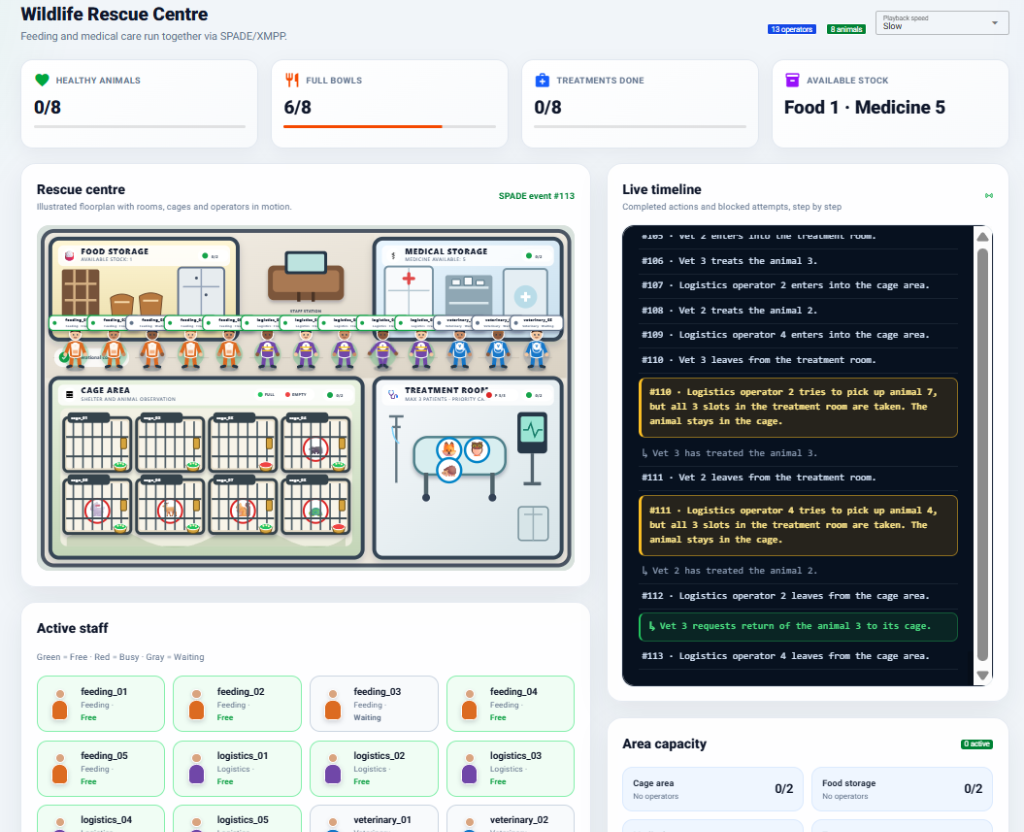
\includegraphics[width=\textwidth]{cras_visualization_dashboard.png}
    \caption{Screenshot of the simulation.}
    \label{fig:visualization_dashboard}
\end{figure}

\section{How to Run the Code}
The system supports two execution modes configurable from the terminal via the main module \texttt{tamagotchi\_wild}.

\subsection{Default Configuration}
If the commands are started without additional parameters, the system automatically loads the predefined baseline configuration:
\begin{itemize}
    \item 5 animals (\texttt{--animals 5})
    \item 7 total operators distributed into:
    \begin{itemize}
        \item 2 veterinarians (\texttt{--veterinary-agents 2})
        \item 3 logistics operators (\texttt{--logistics-agents 3})
        \item 2 feeding operators (\texttt{--feeding-agents 2})
    \end{itemize}
    \item 60 seconds of timeout (\texttt{--timeout 60.0}) and food/medicine stocks automatically calculated to cover requirements. Fundamental to ensure that if an agent gets stuck in a loop, the simulation terminates.
\end{itemize}

\subsection{How to Run}

\subsubsection{Graphical Mode}
Executes the multi-agent simulation and opens the web browser in real time (with default values: 5 animals and 7 operators):
\begin{lstlisting}[language={}]
python -m tamagotchi_wild --gui
\end{lstlisting}

\subsubsection{Headless Mode}
Executes the simulation at maximum speed without a graphical interface:
\begin{lstlisting}[language={}]
python -m tamagotchi_wild
\end{lstlisting}

\subsubsection{Exporting Results to JSON}
Prints the structured summary of tasks to the terminal:
\begin{lstlisting}[language={}]
python -m tamagotchi_wild --json > risultato.json
\end{lstlisting}

\subsection{Custom Parameterization}
If one wishes to customize the parameters, it is possible to override them. At runtime, one can change the values of:
\begin{itemize}
    \item number of animals
    \item number of operators
    \item food and medicine stocks
\end{itemize}
It is also possible to control the GUI; for instance, with \texttt{--gui-port} it is possible to modify the local port of the web server, which defaults to 8080.

\subsubsection{Example with Explicitly Declared Parameters}
\begin{lstlisting}[language={}]
python -m tamagotchi_wild --gui --animals 15 --veterinary-agents 3 --logistics-agents 4 --feeding-agents 3 --timeout 90
\end{lstlisting}

\section{Experimental Results, Anomalies, and Future Work}

\subsection{Simulation Results and Graphical Inspection}
In ordinary tests, the system proves stable and scales successfully with an increasing number of animals (tested up to 40) and operators (tested up to 15). The greatest complexity lies in managing concurrent access to physical spaces and coordination via FIPA-ACL messages.

The NiceGUI interface provides a complete overview of the operational state:

\paragraph{Photo 1 -- Interactive Floor Plan of the Rescue Centre}
Represents the $12 \times 8$ grid divided into the 4 physical areas, tracking in real time the position of operators, cages, and the examination table.
\begin{figure}[htbp]
    \centering
    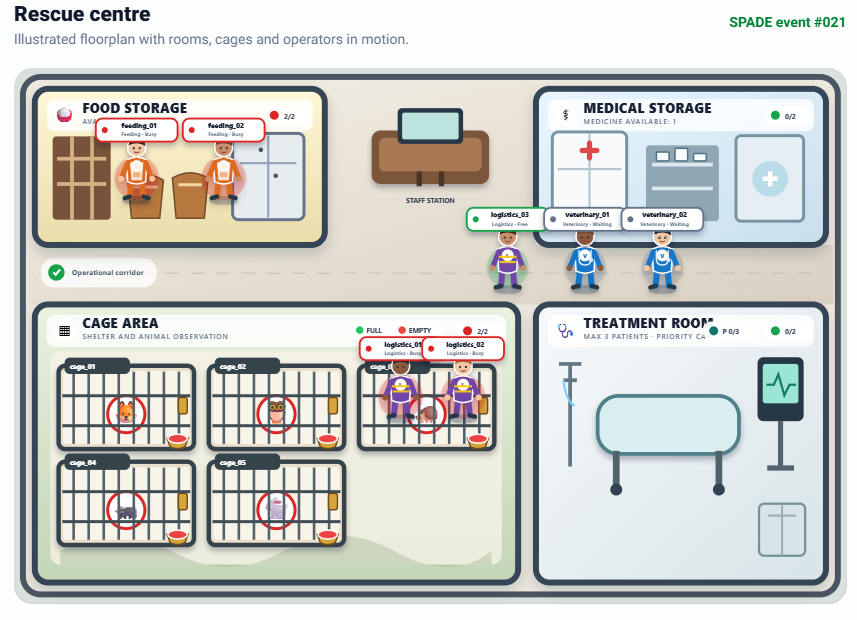
\includegraphics[width=0.85\textwidth]{foto1_rescue_centre.png}
    \label{fig:foto1_rescue_centre}
\end{figure}

\paragraph{Photo 2 -- Live Timeline (Event Log)}
Tracks in chronological order the physical actions validated by the environment (numbered with a \texttt{\#} prefix) and the exchange of FIPA-ACL messages between agents (identified by the arrow prefix $\hookrightarrow$ and a dedicated background).
\begin{figure}[htbp]
    \centering
    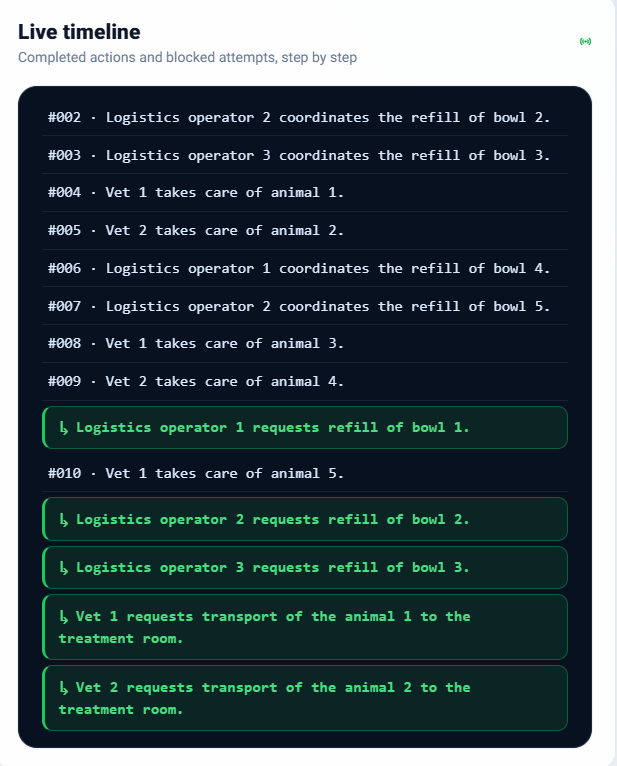
\includegraphics[width=0.85\textwidth]{foto2_live_timeline.png}
    \label{fig:foto2_live_timeline}
\end{figure}

\paragraph{Photo 3 -- Active Staff}
Highlights the status of each agent with color coding: green (\textit{Free}), red (\textit{Busy} with occupied room), and gray (\textit{Waiting}).
\begin{figure}[htbp]
    \centering
    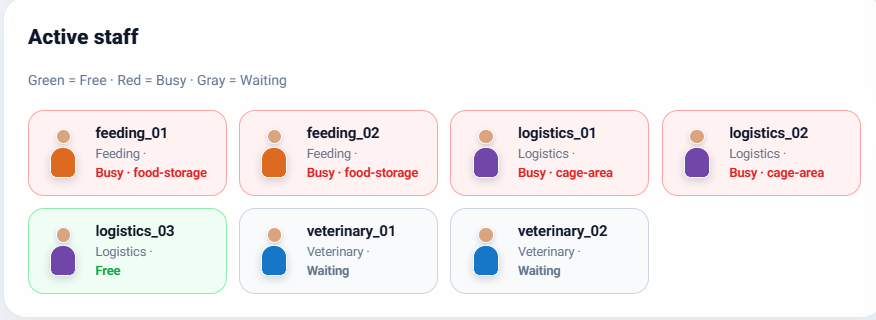
\includegraphics[width=0.85\textwidth]{foto3_active_staff.png}
    \label{fig:foto3_active_staff}
\end{figure}

\paragraph{Photo 4 -- Area Capacity}
Monitors instantaneous occupancy with respect to the physical limit of 2 operators per room.
\begin{figure}[htbp]
    \centering
    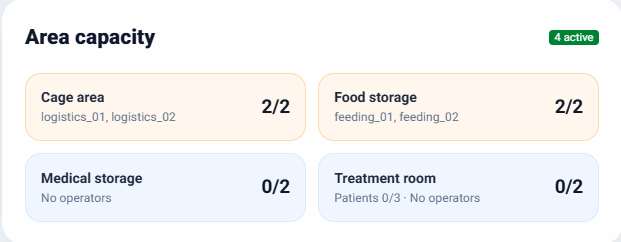
\includegraphics[width=0.75\textwidth]{foto4_area_capacity.png}
    \label{fig:foto4_area_capacity}
\end{figure}

\paragraph{Photo 5 -- Metrics and Remaining Stocks}
Displays overall progress (healthy patients, filled bowls, completed therapies) and the residual level of inventory stocks in storage.
\begin{figure}[htbp]
    \centering
    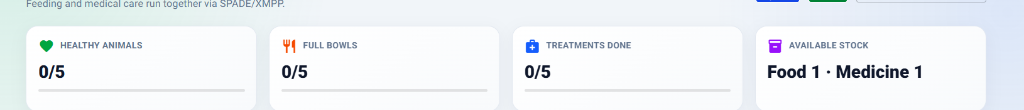
\includegraphics[width=0.85\textwidth]{foto5_metrics_stocks.png}
    \label{fig:foto5_metrics_stocks}
\end{figure}

\subsection{Detected Anomalies and Deadlock Scenarios}

\subsubsection{First Scenario  -- Asymmetric Resources}
\begin{lstlisting}[language={}]
.\.my_sdai\Scripts\python.exe -m tamagotchi_wild --gui --animals 5 --food 2 --medicine 1 --timeout 60.0
\end{lstlisting}
\textbf{Dynamics:} The first 3 patients fully occupy the examination table in the Treatment Room (maximum patient capacity: 3). The only available medicine treats the first patient, who is returned to the cage, freeing a spot on the table that is immediately occupied by another animal.

\noindent\textbf{Livelock / Deadlock Condition:} The animals remaining on the table can neither be treated nor discharged. For the animals still in cages, the logistics operator receives the transport order but finds the treatment room saturated (\textit{treatment room patient capacity is full}). The agent enters an infinite retry loop, resulting in a livelock / deadlock condition where the agents poll endlessly until the global timeout occurs: it accesses the Cage Area, ascertains the impossibility of delivering the patient, releases the room, and retries endlessly until the 60-second timeout occurs.

\subsubsection{Second Scenario -- Total Absence of Resources}
\begin{lstlisting}[language={}]
.\.my_sdai\Scripts\python.exe -m tamagotchi_wild --gui --animals 5 --food 0 --medicine 0 --timeout 60.0
\end{lstlisting}
\textbf{Dynamics:} With zero stocks, the feeding operators declare failure and terminate their activities. On the medical side, the first 3 animals are placed on the examination table. The veterinarians immediately declare \texttt{failure} due to lack of medicine, but do not release the animals.

\noindent\textbf{Two-Agent Livelock / Deadlock:} The 3 examination table spots remain permanently occupied. \textbf{Two logistics operators end up simultaneously in an infinite loop of accessing the Cage Area}, continually attempting to retrieve the 4th and 5th animals without being able to deliver them to the saturated treatment room, causing a livelock / deadlock condition where the agents poll endlessly until the global timeout occurs.

\subsubsection{Primary Root Cause of All Deadlocks and Livelocks}
All observed deadlocks and livelocks are traceable to a single cause: \textbf{the total and definitive capacity saturation of the examination table in the treatment room (i.e., all 3 patient spots occupied)}.

In the BDI plan of the veterinarian (\texttt{veterinary.asl}), the return transport request (\texttt{request\_medical\_transport(..., return)}) is triggered exclusively upon therapeutic success (\texttt{treatment\_succeeded}). In case of failure due to exhausted stocks (\texttt{medical\_failed}), the cycle closes without requesting the return of the animal. Consequently, untreated patients remain trapped on the examination table indefinitely, saturating room capacity and trapping logistics agents in cyclic delivery attempts.

\subsection{Proposals for Improvement}
\begin{itemize}
    \item \textbf{Mandatory Return upon Therapy Failure}: Modify \texttt{veterinary.asl} so that treatment failure also triggers a return transport request, immediately freeing the spot on the examination table.
    \item \textbf{Preventive Stock Verification}: Condition the transport of an animal to the medical room on prior verification of available doses in storage.
\end{itemize}

\bigskip
\noindent\textbf{Concluding Remarks.} Although the system represents a prototype with substantial room for extension and refinement, the development of the project has been a highly formative and stimulating experience, providing first-hand engagement with the concrete engineering challenges posed by integrating symbolic artificial intelligence (BDI) with asynchronous distributed architectures.

\end{document}


